\documentclass[12pt]{article}
\usepackage{preamble}

\pagestyle{fancy}
\fancyhead[LO,LE]{Теория вероятности}
\fancyhead[CO,CE]{22.10.2024}
\fancyhead[RO,RE]{Лекции Блаженова А. В.}

\fancyfoot[L]{\scriptsize исходники найдутся тут: \\ \url{https://github.com/pelmesh619/itmo_conspects} \Cat}

\begin{document}
    \subsection{Функция распределения}

    \Def Функция распределения $F_\xi(x)$ случайной величины $\xi$ называется функция $F_\xi(x) = P(\xi < x)$

    $F(x)$ - вероятность попадания в этот интервал

    \Ex $\xi \in B_p$ \qquad \begin{tabular}{c|c|c}
        $\xi$ & 0 & 1 \\ \hline
        $p$ & $1 - p$ & $p$ \\
    \end{tabular} \qquad $F_\xi(x) = \begin{cases}0 \quad x \leq 0, \\ 1 - p \quad 0 < x \leq 1, \\ 1 \quad x > 1\end{cases}$

    \subsubsection{Свойства функции распределения}

    1) $F(x)$ ограничена $0 \leq F(x) \leq 1$

    2) $F(x)$ неубывающая функция: $x_1 < x_2 \Longrightarrow F(x_1) \leq F(x_2)$ 

    \begin{MyProof}
        $x_1 < x_2 \Longrightarrow \{\xi < x_1\} \subset \{\xi < x_2\} \Longrightarrow p(\xi < x_1) \leq p(\xi < x_2)$, то есть $F(x_1) \leq F(x_2)$
    \end{MyProof}

    3) $p(\alpha \leq \xi < \beta) = F(\beta) - F(\alpha)$

    \begin{MyProof}
        $p(\xi < \beta) = p(\xi < \alpha) + p(\alpha \leq \xi < \beta) \Longrightarrow F(\beta) = F(\alpha) + p(\alpha \leq \xi < \beta)$
    \end{MyProof}
    
    \Notas Функция распределения $F(x)$ - вероятность попадания в интервал $(-\infty; x)$. Так как Борелевская $\sigma$-алгебра порождается такими интервалами,
    то распределение полностью задается этой функцией

    4) $\lim_{x \to -\infty} F(x) = 0; \quad \lim_{x \to +\infty} F(x) = 1$

    \begin{MyProof}
        Так как $F(x)$ монотонна и ограничена, то эти пределы существуют. Поэтому достаточно доказать эти пределы для некоторой последовательности $x_n \to \pm \infty$

        $\letsymbol A_n = \{n - 1 \leq \xi < n, n \in v\}$ - несовместные события, так как $\Real = \bigunion_{n = -\infty}^\infty A_n$, то
        по аксиоме счетной аддитивности, вероятность $p(\xi \in \Real) = 1 = \sum_{n = -\infty}^\infty P(A_n) = \lim_{N \to \infty} \sum_{n = -N}^N p(n - 1 \leq \xi < n) = 
        \lim_{N \to \infty} \sum_{n = -N}^N (F(n) - F(n - 1)) = \lim_{N \to \infty} (F(N) - F(-N - 1)) = \lim_{N \to \infty} F(N) - \lim_{N \to -\infty} F(N) = 1$

        $\Longrightarrow \lim_{N \to \infty} F(N) = 1 + \lim_{N \to -\infty} F(N) $

        Так как $\lim_{N \to \infty} F(N) \leq 1$ и $\lim_{N \to -\infty} F(N) \geq 0$, то $\lim_{N \to \infty} F(N) = 1$ и $\lim_{N \to -\infty} = 0$
    \end{MyProof}
    
    5) $F(x)$ непрерывна слева: $F(x_0 - 0) = F(x_0)$

    \begin{MyProof}
        Этот предел существует в силу монотонности и ограниченности функции, поэтому рассмотрим последовательность событий $B_n = \{x_0 - \frac{1}{n} \leq \xi < x_0, n \in \mathrm{Z}\}$

        Так как $B_1 \supset B_2 \supset \dots \supset B_n \supset \dots$ и $\bigcap_{n = 1}^\infty B_n = \emptyset$

        То по аксиоме непрерывности $p(B_n) \to 0$

        $P(B_n) = F(x_0) - F(x_0 - \frac{1}{n}) \rightarrow 0$

        $F(x_0 - \frac{1}{n}) \to F(x_0)$

        $\lim_{x \to x_0 - 0} F(x) = F(x_0)$
    \end{MyProof}
    
    6) Скачок в точке $x_0$ равен вероятности попадания в данную точку: $F(x_0 + 0) - F(x_0) = p(\xi = x_0)$ или $F(x_0 + 0) = p(\xi = x_0) + p(\xi < x_0) = p(\xi \leq x_0)$

    
    \begin{MyProof}
        Этот предел существует в силу монотонности и ограниченности функции, поэтому рассмотрим последовательность событий $C_n = \{x_0 \leq \xi < x_0 + \frac{1}{n}, n \in \mathrm{Z}\}$

        Так как $C_1 \supset C_2 \supset \dots \supset C_n \supset \dots$ и $\bigcap_{n = 1}^\infty C_n = \emptyset$

        То по аксиоме непрерывности $p(C_n) \to 0$

        $P(C_n) = F(x_0 + \frac{1}{n}) - F(x_0) \rightarrow 0$

        $p(x_0 \leq \xi < x_0 + \frac{1}{n}) + p(\xi = x_0) \rightarrow p(\xi = x_0)$

        $F(x_0 + \frac{1}{n}) - F(x_0) \to p(\xi = x_0)$

        $F(x_0 + 0) - F(x_0) \to p(\xi = x_0)$
    \end{MyProof}
    
    7) Если функция распределения непрерывна в точке $x = x_0$, то очевидно, что вероятность попадания в эту точка $p(\xi = x_0) = 0$ (следствие из 6 пункта)
    
    8) Если $F(x)$ непрерывна $\forall x \in \Real$, то $p(\alpha \leq \xi < \beta) = p(\alpha < \xi < \beta) = p(\alpha \leq \xi \leq \beta) = p(\alpha < \xi \leq \beta) = F(\beta) - F(\alpha)$
    
    \begin{MyTheorem}
        \Ths Случайная величина $\xi$ имеет дискретное распределение тогда и только тогда, когда ее функция распределения имеет ступенчатый вид
    \end{MyTheorem}

    \subsection{Абсолютно непрерывное распределение}

    \Def Случайная величина $\xi$ имеет абсолютно непрерывное распределение, если существует $f_\xi(x)$ такая, что $\forall B \in \mathcal{B}(\Real)
    \ p(\xi \in B) = \int_B f_\xi(x)dx$

    Функция $f_\xi$ называется плотностью распределения случайной величины

    (в определении использует интеграл Лебега, так как $B$ может быть не просто интервалом на $\Real$)

    \subsubsection{Свойства плотности и функции распределения абсолютно непрерывного распределения}

    1) Вероятносто-геометрический смысл плотности: $p(\alpha \leq \xi < \beta) = \int_{\alpha}^\beta f_\xi(x) dx$

    2) Условие нормировки: $\int_{-\infty}^{+\infty} f_\xi(x)dx = 1$

    \begin{MyProof}
        Из определения, если $B = \Real$
    \end{MyProof}

    3) $F_\xi(x) = \int_B f_\xi(x)dx$

    \begin{MyProof}
        Если $B = (-\infty; x)$, то $F_\xi(x) = p(\xi \in (-\infty; x)) = \int_{-\infty}^x f_\xi(x)dx$
    \end{MyProof}

    4) $F_\xi(x)$ непрерывна 
    
    \begin{MyProof}
        Из свойства непрерывности интеграла с верхним переменным пределом
    \end{MyProof}

    5) $F_\xi(x)$ дифференцируема почти везде и $f_\xi(x) = F^\prime_\xi(x)$ для почти всех $x$
    
    \begin{MyProof}
        По теореме Барроу
    \end{MyProof}

    6) $f_\xi(x) \geq 0$ по определению и как производная неубывающей $F_\xi(x)$

    7) $p(\xi = x) = 0 \ \forall x \in \Real$ - так как $F_\xi(x)$ непрерывна

    8) $p(\alpha \leq \xi < \beta) = p(\alpha < \xi < \beta) = p(\alpha \leq \xi \leq \beta) = p(\alpha < \xi \leq \beta) = F(\beta) - F(\alpha)$

    9) \Ths Если $f(x) \leq 0$ и $\int_{-\infty}^{\infty} f(x)dx$ (выполнены свойства 2 и 6), то $f(x)$ - плотность некоторого распределения

    \subsubsection{Числовые характеристики}

    \Def Математическим ожиданием $E\xi$ случайной абсолютно непрерывной величины $\xi$ называется величина $E\xi = \int_{-\infty}^{\infty} xf_\xi(x) dx$ 
    при условии, что данный интеграл сходится абсолютно, то есть $\int_{-\infty}^\infty |x|f_\xi(x)dx < \infty$

    \Def Дисперсией $D\xi$ случайной величины $\xi$ называется величина $D\xi = E(\xi - E\xi)^2 = \int_{-\infty}^\infty (x - E\xi)^2 f_\xi(x) dx$ при условии,
    что данный интеграл сходится

    \Notas Вычислять удобно по формуле $D\xi = E\xi^2 - (E\xi)^2 = \int_{-\infty}^\infty x^2 f_\xi(x)dx - (E\xi)^2$

    \Def Среднее квадратическое отклонение $\sigma_\xi = \sqrt{D\xi}$ определяется, как корень дисперсии

    Смысл этих величин такой же, как и при дискретном распределении. Также свойства аналогичны тем, что и при дискретном распределении

    \subsubsection{Другие числовые характеристики}

    $m_k = E\xi^k = \int_{-\infty}^\infty x^k f_\xi(x)dx$ - момент $k$-ого порядка

    $\mu_k = E(\xi - E\xi)^k = \int_{-\infty}^\infty (x - E\xi)^k f_\xi(x)dx$ - центральный момент $k$-ого порядка

    \Def Медианой $Me$ абсолютно непрерывной случайной величины $\xi$ называется значение случайной величины $\xi$, такое что $p(\xi < Me) = p(\xi > Me) = \frac{1}{2}$

    \Def Модой $Mo$ случайной величины $\xi$ называется точка локального максимума плотности

    \subsection{Сингулярное распределение}

    \Def Случайная величина $\xi$ имеет случайное распределение, если $\exists B$ - Борелевское множество с нулевой мерой Лебега $\lambda(B) = 0$, такое что $p(\xi \in B) \in 1$, но $P(\xi = x) = 0 \ \, \forall x \in B$

    \Nota Такое Борелевское множество состоит из несчетного множества точек, так как в протичном случае по аксиоме счетной аддитивности $p(\xi \in B) = 0$. То есть 
    при сингулярном распределении случайная величина $\xi$ распределена на несчетном множестве меры 0

    \Notas Так как $p(\xi = x) = 0 \  \forall x$, $F_\xi$ непрерывна.

    \smallvspace
    
    \begin{minipage}{\textwidth}
        \begin{wrapfigure}{r}{0pt}
            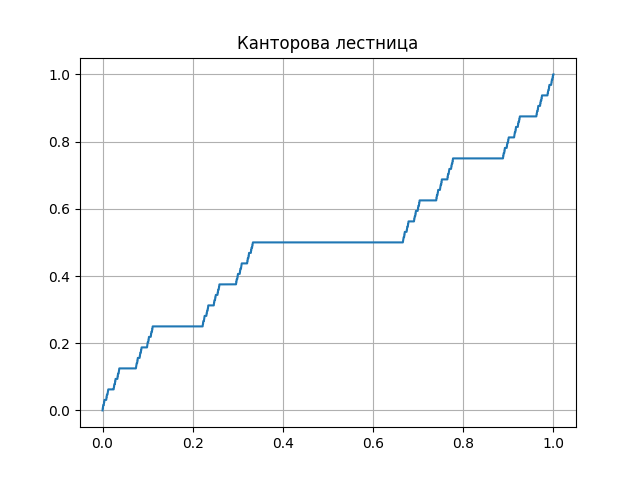
\includegraphics[width=7cm]{probtheory/images/probtheory_2024_10_22_1}
        \end{wrapfigure}

        % import matplotlib.pyplot as plt
        % import numpy

        % cache = {}

        % def f(x, c=0):
        %     if c >= 100:
        %         return x

        %     if x not in cache:
        %         cache[x] = 0 if x <= 0 else \
        %             1/2 * f(3 * x, c+1) if x <= 1/3 else \
        %             1/2 if x <= 2/3 else \
        %             1/2 + 1/2 * f(3 * x - 2, c+1) if x <= 1 else \
        %             1 

        %     return cache[x]

        % x_domain = numpy.arange(0, 1.001, 0.0001)
        % plt.plot(x_domain, [f(i) for i in x_domain])
        % plt.title("Канторова лестница")
        % plt.grid(True)
        % plt.show()

        \Exs Сингулярное распределение получим, если возьмем случайную величину, функция распределения которой - 
        лестница Кантора
    
        $F_\xi(x) = \begin{cases}0 \quad x \leq 0, \\ \frac{1}{2}F(3x) \quad 0 < x \leq \frac{1}{3}, \\ \frac{1}{2} \quad \frac{1}{3} < x \leq \frac{2}{3}, \\ \frac{1}{2} + \frac{1}{2}F(3x - 2) \quad \frac{2}{3} < x \leq 1, \\ 1 \quad x > 1\end{cases}$
    \end{minipage}

    \begin{MyTheorem}
        \ThNs{Лебега}

        $\letsymbol F_\xi(x)$ - функция распределения $\xi$. Тогда $F_\xi(x) = p_1 F_1(x) + p_2 F_2(x) + p_3 F_3(x)$, где $p_1 + p_2 + p_3 = 1$

        $F_1$ - функция дискретного распределения

        $F_2$ - функция абсолютно непрерывного распределения

        $F_3$ - функция сингулярного распределения

        То есть существуют только дискретное, абсолютно непрерывное, сингулярное распределения и их смеси
    \end{MyTheorem}


\end{document}
